\documentclass[12pt,letterpaper]{article}
\usepackage[utf8]{inputenc}
\usepackage[spanish]{babel}
\usepackage{graphicx}
\usepackage{geometry}
\usepackage{parskip}
\usepackage{float}
\usepackage{titlesec}
\usepackage{hyperref}
\usepackage{multicol}
\usepackage{caption}

% Quitar numeración de secciones y subsecciones
\setcounter{secnumdepth}{0}

% Reducir espacio antes y después de títulos de sección
\titlespacing*{\section}{0pt}{10pt}{4pt}
\titlespacing*{\subsection}{0pt}{8pt}{3pt}

\geometry{top=2.5cm, bottom=2.5cm, left=3cm, right=2.5cm}

\begin{document}

% ─── PORTADA ───────────────────────────────────────────────────────────────────
\thispagestyle{empty}

\begin{center}
    
\includegraphics[scale=0.8]{encabezadoportada.png}
\end{center}
\vspace{0.5cm}
\begin{center}
    \LARGE{INSTITUTO TECNOLÓGICO SUPERIOR}\\
    \LARGE{DE SAN PEDRO DE LAS COLONIAS}
\end{center}
\vspace{0.5cm}
\begin{center}
    
\includegraphics[scale=0.1]{LOGO-PRINCIPAL.png}
\end{center}
\vspace{0.8cm}

\hrule
\begin{center}
    \textbf{\Large{INGENIERÍA EN SISTEMAS COMPUTACIONALES}}\\[2pt]
    \textbf{\Large{Redes de Computadoras}}
\end{center}
\hrule

\vspace{0.6cm}

\begin{center}
    \textbf{\Large{Práctica: Elaboración de cable Ethernet}}\\
\end{center}

\vspace{0.5cm}
\begin{center}
    \textsc{\large{Maestra:}} \\
    \textsc{\large{Niria González Ortiz}}
\end{center}

\vspace{0.5cm}
\begin{center}
    \textsc{\large{Estudiante}}\\[4pt]
    \large{Alexis Alvarado Gómez}\\
    \vspace{0.2cm}
    \large{Número de control}\\
    \large{231000176}
\end{center}

\vfill

\begin{center}
    \large{San Pedro, Coahuila de Zaragoza a 09 de mayo del 2026.}
\end{center}

\newpage

% ─── OBJETIVO ──────────────────────────────────────────────────────────────────
\section{Objetivo}

Aprender a fabricar un cable de red Ethernet de tipo directo utilizando el
estándar T568B, identificando correctamente el orden de los colores de los
hilos y aplicando el uso adecuado de las herramientas como la ponchadora
y el pelacables.

% ─── INTRODUCCIÓN ──────────────────────────────────────────────────────────────
\section{Introducción}

En esta práctica aprendimos a hacer un cable de red Ethernet de tipo directo
usando el estándar T568B. Un cable Ethernet sirve para conectar dispositivos
a una red local, como una computadora a un router o switch.
Para hacerlo necesitamos cable UTP CAT6, conectores RJ45 y una ponchadora.
El proceso es sencillo: se pela el cable, se ordenan los hilos por color y
se poncha el conector.

% ─── MATERIALES ────────────────────────────────────────────────────────────────
\section{Materiales}

\begin{itemize}
    \item Cable UTP CAT6 (la longitud que necesites)
    \item 2 conectores RJ45
    \item Ponchadora (crimpadora)
    \item Pelacables
    \item Tijeras o navaja
\end{itemize}

\begin{figure}[H]
    \centering
    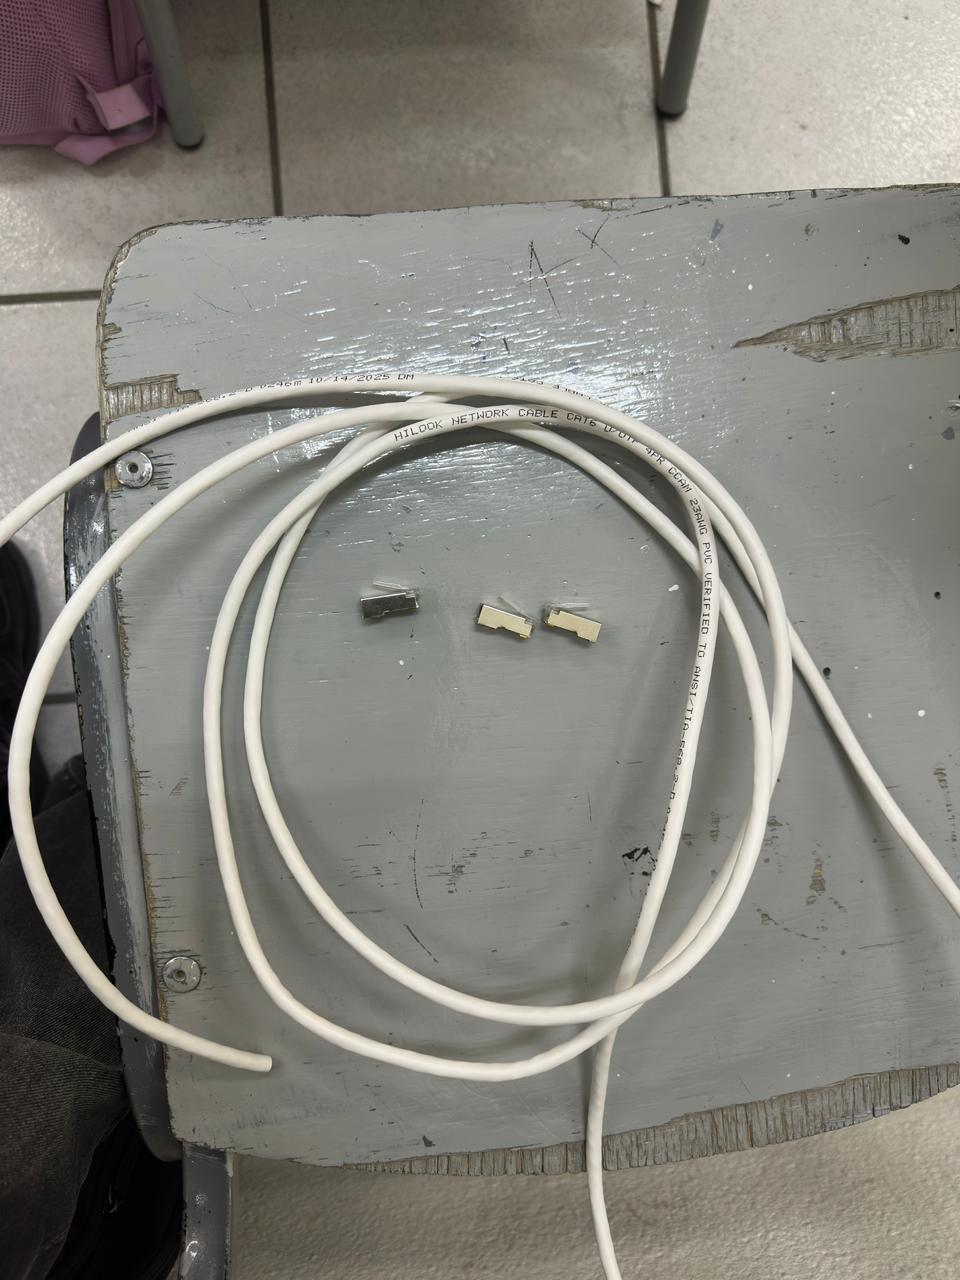
\includegraphics[width=0.40\textwidth]{1_materiales.jpg}
    \caption*{Cable CAT6 y conectores RJ45 listos para usar.}
\end{figure}

% ─── DESARROLLO ────────────────────────────────────────────────────────────────
\section{Desarrollo}

\subsection{Paso 1 – Pelar el cable}

Con el pelacables se quita unos 2 o 3 cm de la cubierta exterior del cable
para dejar al descubierto los 4 pares de hilos trenzados.
Hay que tener cuidado de no cortar los hilos internos.

\begin{figure}[H]
    \centering
    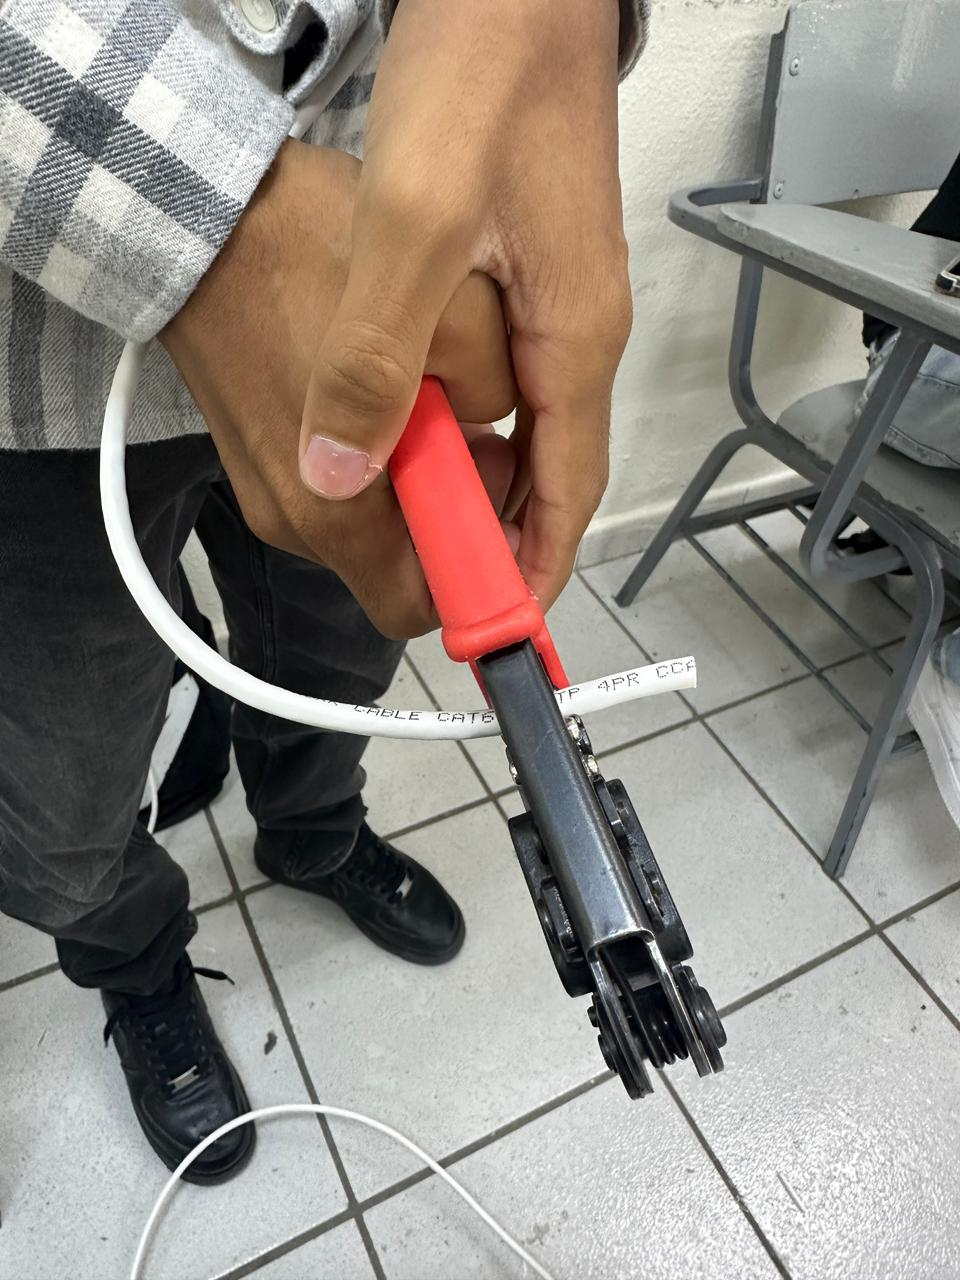
\includegraphics[width=0.85\textwidth]{2_pelar.jpg}
    \caption*{Usando el pelacables para retirar la cubierta exterior del cable.}
\end{figure}

\newpage

\subsection{Paso 2 – Separar y desenredar los pares}

Una vez pelado el cable, se separan los 4 pares trenzados. Cada par tiene
dos hilos: uno de color sólido y uno blanco con rayas del mismo color.
Se desenredan con cuidado para poder ordenarlos.

\begin{figure}[H]
    \centering
    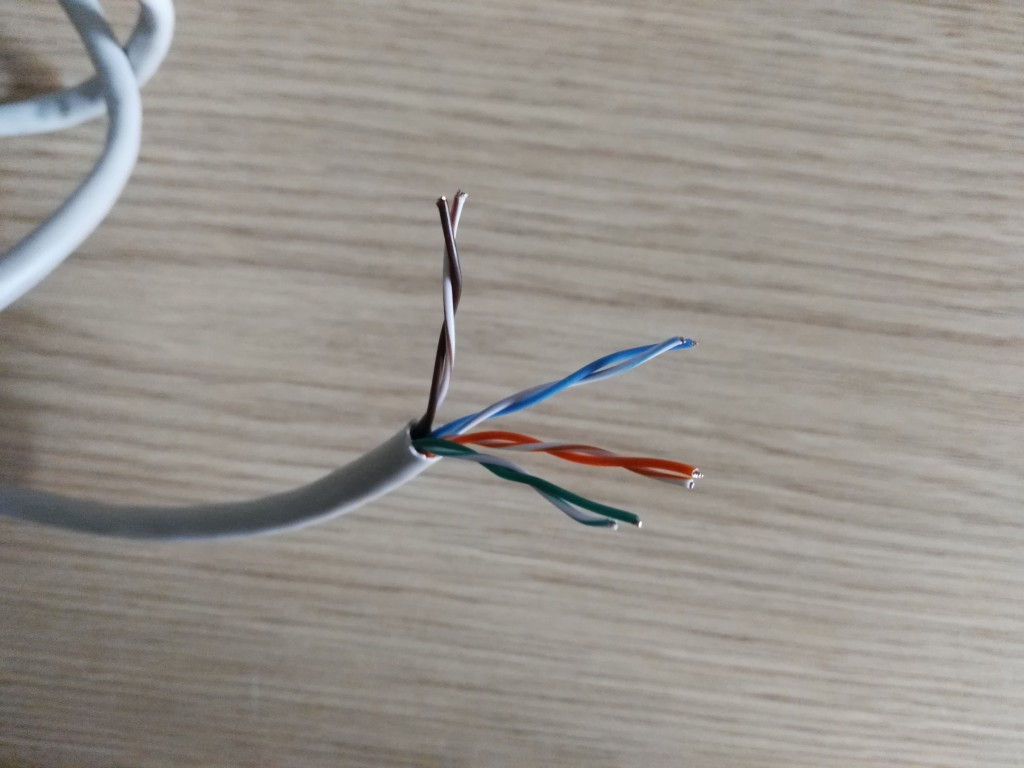
\includegraphics[width=0.85\textwidth]{3_pares.jpg}
    \caption*{Los 4 pares de hilos trenzados ya separados.}
\end{figure}

\newpage

\subsection{Paso 3 – Ordenar los hilos (estándar T568B)}

Los 8 hilos se acomodan en este orden de izquierda a derecha según el estándar T568B:

\begin{center}
\begin{tabular}{|c|c|l|}
\hline
\textbf{Pin} & \textbf{Color} & \textbf{Descripción} \\
\hline
1 & Blanco/Naranja & Par naranja \\
2 & Naranja        & Par naranja \\
3 & Blanco/Verde   & Par verde   \\
4 & Azul           & Par azul    \\
5 & Blanco/Azul    & Par azul    \\
6 & Verde          & Par verde   \\
7 & Blanco/Café    & Par café    \\
8 & Café           & Par café    \\
\hline
\end{tabular}
\end{center}

\begin{figure}[H]
    \centering
    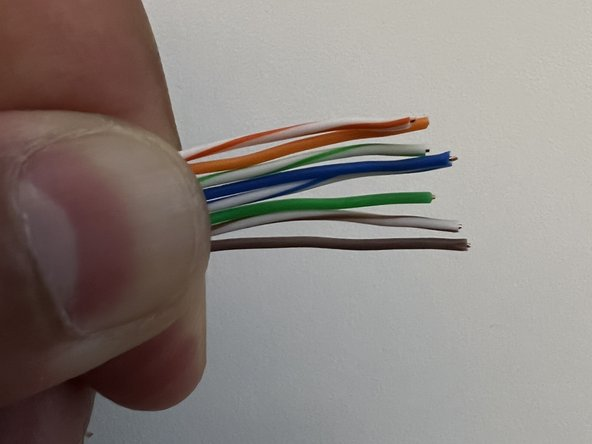
\includegraphics[width=0.85\textwidth]{4_ordenar.jpg}
    \caption*{Hilos alineados en el orden correcto del estándar T568B.}
\end{figure}

\newpage

\subsection{Paso 4 – Insertar los hilos en el conector RJ45}

Con los hilos ya ordenados y parejos, se meten dentro del conector RJ45.
Hay que empujarlos bien hasta el fondo para que cada hilo llegue a su pin
correspondiente. Se puede ver a través del plástico transparente del conector
que todos los hilos llegaron hasta el final.

\begin{figure}[H]
    \centering
    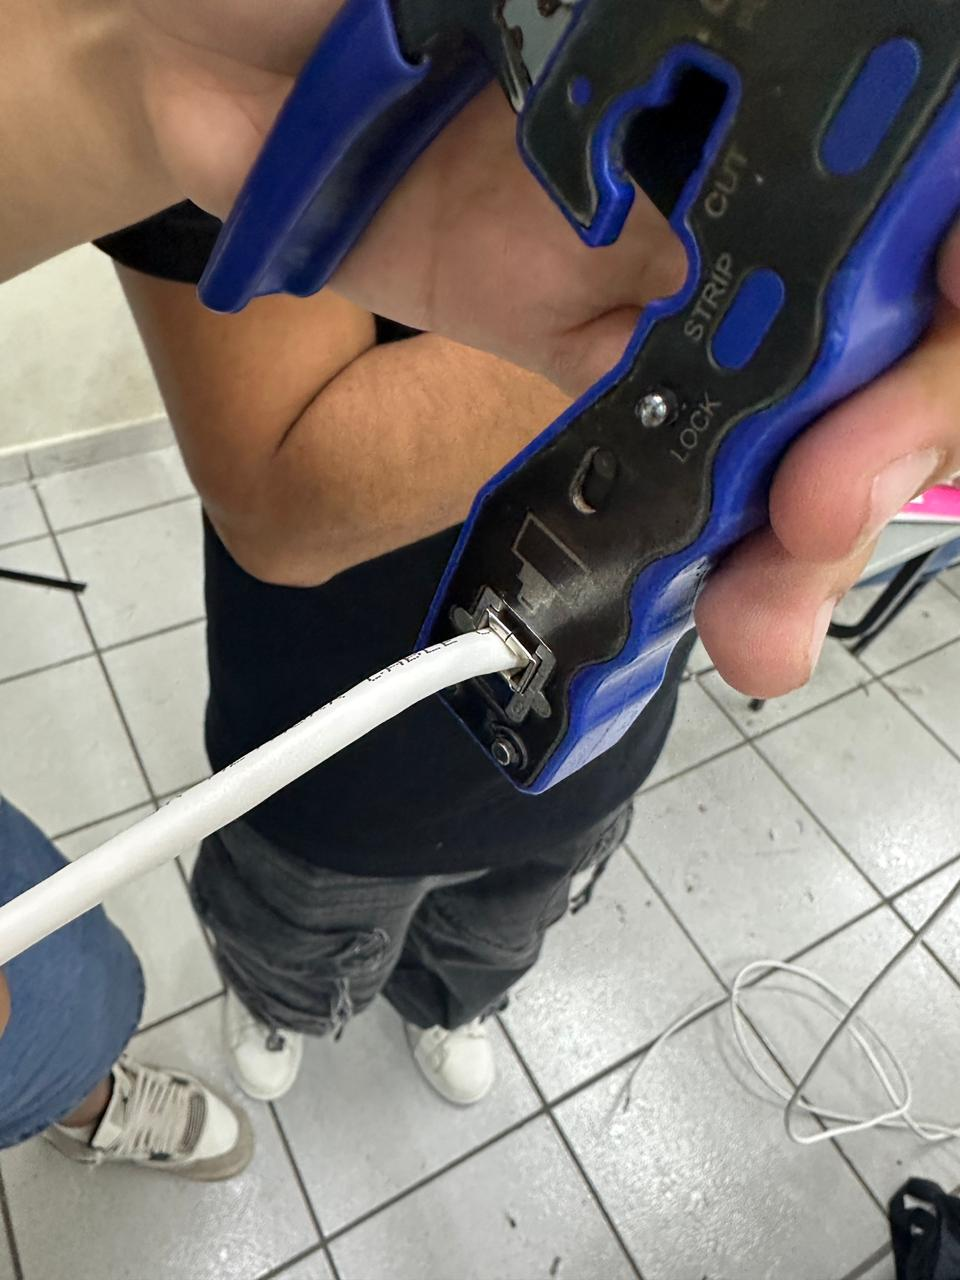
\includegraphics[width=0.85\textwidth]{5_conector.jpg}
    \caption*{Hilos insertados correctamente en el conector RJ45.}
\end{figure}

\newpage

\subsection{Paso 5 – Ponchar el conector}

Se mete el conector en la ponchadora y se aprieta con fuerza. Esto hace que
los pines del conector perforen el aislante de cada hilo y hagan contacto
eléctrico. También fija la cubierta del cable para que no se jale.
Se repite el mismo proceso en el otro extremo con el mismo orden de colores
(T568B -- T568B = cable directo).

\begin{figure}[H]
    \centering
    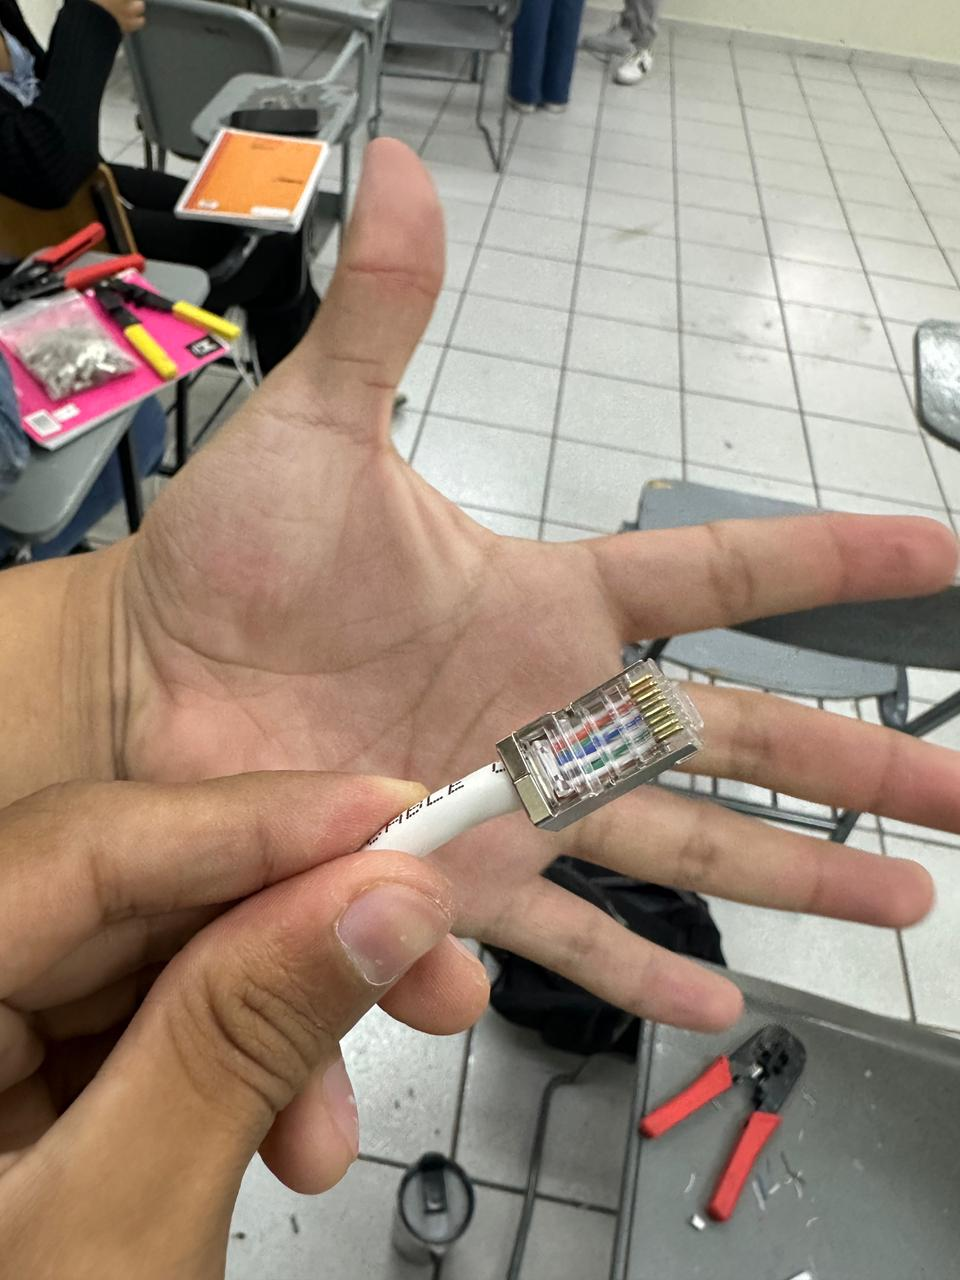
\includegraphics[width=0.85\textwidth]{6_ponchar.jpg}
    \caption*{Ponchando el conector RJ45 con la crimpadora.}
\end{figure}

\newpage

% ─── RESULTADOS ────────────────────────────────────────────────────────────────
\section{Resultados}

Al terminar los dos extremos del cable, lo probamos conectándolo entre dos
dispositivos. La conexión funcionó correctamente, lo que indica que los hilos
quedaron bien ordenados y los conectores bien ponchados.

\begin{figure}[H]
    \centering
    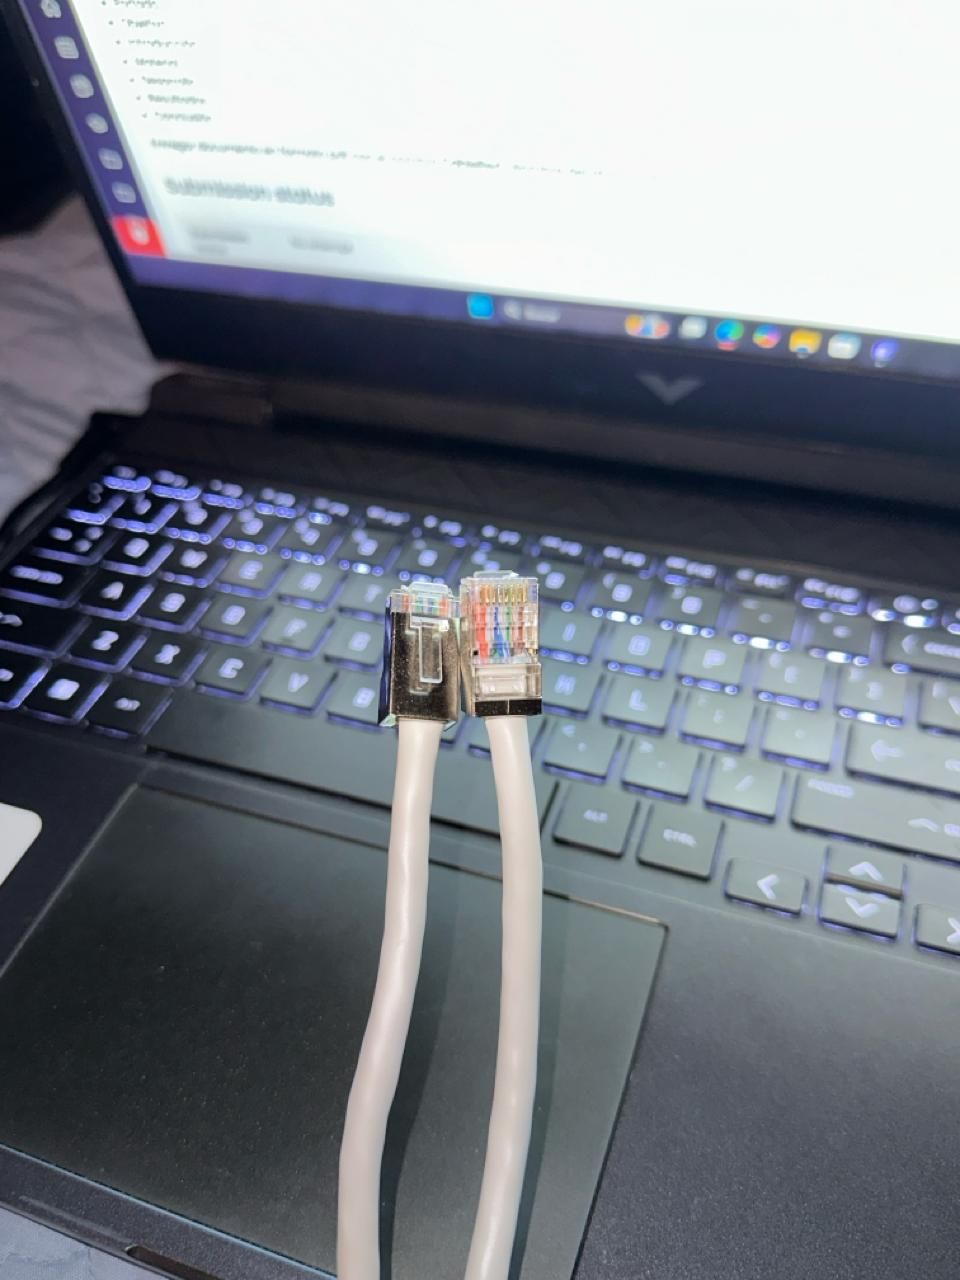
\includegraphics[width=0.85\textwidth]{7_resultados.jpg}
    \caption*{Los dos extremos del cable terminados con sus conectores RJ45 ponchados.}
\end{figure}

% ─── CONCLUSIÓN ────────────────────────────────────────────────────────────────
\section{Conclusión}

Hacer un cable Ethernet no es tan difícil como parece. Lo más importante es
respetar el orden de los colores según el estándar T568B y asegurarse de que
todos los hilos lleguen hasta el fondo del conector antes de ponchar.
Con esta práctica aprendimos cómo se fabrican los cables de red que usamos
todos los días y entendimos por qué el orden de los colores importa para que
la comunicación funcione bien.

\end{document}
